\documentclass[11pt]{article}
\usepackage[margin=1in]{geometry}
\usepackage{booktabs,multirow,graphicx,amsmath,amssymb,xcolor,xurl,hyperref,natbib}
\newcommand{\pending}[1]{\textcolor{red}{[#1]}}
\newcommand{\authorinfo}[1]{\textcolor{blue}{[#1]}}

\title{Why Self-Arbitration Looks Like Guessing:\\A Diagnostic Study of Small Language Models}
\author{Manh Khang Tran\\Independent researcher\\[2pt]
\small\url{https://github.com/KhangTranManh/Self-Correction-Model}}
\date{Preprint, October 2026\\[2pt]
\small DOI: \href{https://doi.org/10.5281/zenodo.23541462}{10.5281/zenodo.23541462}}

\hypersetup{pdftitle={Why Self-Arbitration Looks Like Guessing: A Diagnostic Study of Small Language Models},
  pdfauthor={Tran, Manh Khang}, pdfsubject={doi:10.5281/zenodo.23541462}}
\begin{document}
\maketitle

\begin{abstract}
When a 7B language model solves a problem twice, gets two different answers, and is asked which of its own
solutions is right, it looks close to guessing: judged in a single presentation order, it picks the correct
solution 45--64\% of the time. We ask whether this reflects a lack of skill or the way it is measured. On
self-generated solution pairs with deterministic labels (four models from three families, four math datasets,
both presentation orders), a skill index that cancels pure position bias is clearly positive in every cell we
measured: 4/4 preregistered endpoint cells (Llama-3.1-8B, Mistral-7B $\times$ ASDiv, MATH levels 1--3) and
16/16 descriptive cells. Decomposing the single-order shortfall shows that position bias costs only 0--2.5
accuracy points (at most 1.9 under a probit link); most of the gap comes from the judge not making a valid
choice between the two solutions --- writing its choice in an unreadable format, giving a third answer, or
being cut off at the token limit while looping. Only 51--90\% of single-order judgments are valid choices. Part of this is an
answer-format artefact: re-reading the judge's final line raises the untrained Qwen2.5-7B-Instruct from
45--64\% to 72--88\%. For Qwen the split between position bias and invalid choices is not clean: it fails to
choose more often when the correct solution is shown second, so part of its position preference appears as
invalid choices. Averaging verdict probabilities over both orders, the debiasing method of
\citet{ren2023selfeval}, adds little (1/4 preregistered cells reach $\geq$3 points). Hidden states carry a
right/wrong signal in all four models, but beat simple surface features consistently only for the
self-correction model. At the system level, using the judge's verdict loses to majority voting over three
samples in 15/16 cells; falling back to a third sample when the two orders disagree only ties three-sample
voting, and every two-candidate strategy loses to voting over five.
\end{abstract}

\section{Introduction}
Self-correction involves three steps: noticing that an answer may be wrong, deciding which of several
candidate answers is right, and repairing the answer. Prior work finds that small and medium models struggle
to self-correct reasoning without external feedback \citep{huang2023cannot}, and that the bottleneck is
locating errors rather than fixing them \citep{tyen2024find}. We study the middle step, \emph{arbitration}:
given two of its own solutions with different final answers, can the model tell which one is right?

Arbitration is usually scored in a single presentation order. Position bias is well documented in
LLM-as-a-judge settings \citep{zheng2023judging,wang2024fair,shi2024judging}, but it is rarely separated from
skill when a model judges its own solutions. We ask whether the conclusion ``the model is guessing'' reflects a
lack of skill or the measurement.

\paragraph{Contributions.}
(i) A decomposition of single-order arbitration accuracy into skill, position bias and \emph{invalid choices},
applied to self-generated solution pairs with deterministic labels.
(ii) A preregistered test on two model families and two fresh datasets showing that the skill is real and
general (E1, 4/4 cells), while order-averaging adds little (E2, 1/4 cells).
(iii) Evidence that the dominant cost of single-order arbitration is not position bias but the judge failing
to make a valid choice (format errors, third answers, truncation while looping), with a seven-way
classification of judgment outcomes and bounds that do not depend on the model of the decomposition.
(iv) A representation-level analysis showing a right/wrong signal in hidden states that is only partly
distinct from surface cues, and a practical comparison with majority voting.

\section{Related work}
\paragraph{Self-correction.} Intrinsic self-correction often fails to improve reasoning
\citep{huang2023cannot}; models find errors poorly but fix them when told where they are \citep{tyen2024find}.
Training methods such as SCoRe \citep{kumar2025score} and RISE \citep{qu2024rise} teach multi-turn
self-correction. We isolate arbitration between two of the model's own solutions.
\paragraph{LLM judges and position bias.} LLM judges prefer answers by position
\citep{zheng2023judging,wang2024fair}; the size of the bias depends on the quality gap between candidates
\citep{shi2024judging}. JudgeBench \citep{tan2025judgebench} scores judges on pairs with objective labels and
finds strong judges near chance; J1 \citep{whitehouse2026j1} and permutation-aware RL
\citep{pagrpo2026} train judges for order consistency. Self-preference is a competing explanation when a model
judges its own text \citep{panickssery2024recognize}.
\paragraph{Selecting among own samples.} Universal self-consistency lets the model pick the most consistent
answer \citep{chen2023usc}. \citet{ren2023selfeval} report that averaging letter probabilities over shuffled
orders barely changes selection accuracy (+0.5--0.6 points); we measure the same quantity in our setting.
\paragraph{Probing for correctness.} Hidden states encode the truth of statements
\citep{burns2023latent,azaria2023lying,marks2023geometry} and models can encode the right answer while
producing a wrong one, with probes that transfer poorly across datasets \citep{orgad2025know}; P(True)-style
self-evaluation is calibrated in large models \citep{kadavath2022know}.
\paragraph{Positioning.} We do not propose order swapping (it is standard). We use it to separate bias from
skill on self-generated pairs, show that the remaining shortfall is mostly invalid choices, and connect the
output-level picture to hidden states under a preregistered protocol.

\section{Setup}
\paragraph{Models.} Self\_Correction\_v1, a Qwen2.5-7B-Instruct fine-tuned for self-correction (one SFT
stage on verified correction traces); its untrained parent Qwen2.5-7B-Instruct; Llama-3.1-8B-Instruct; and
Mistral-7B-Instruct-v0.3. Two LoRA judges trained by DPO on order-swapped data (p12, p13b) are used only in the
single-model analysis (\S\ref{sec:sc}).
\paragraph{Data.} GSM8K test problems 750--1318 \citep{cobbe2021gsm8k} (561; 519 after removing 42 that
appeared in an earlier evaluation-only run), SVAMP (960) \citep{patel2021svamp}, and two fresh datasets frozen
before any generation: ASDiv (822) \citep{miao2020asdiv} and MATH levels 1--3 with numeric answers (785)
\citep{hendrycks2021math}. No problem overlaps earlier phases or training data.
\paragraph{Pairs.} Each model samples five solutions per problem (temperature 0.7); the first 768 tokens are
used. Pairs $(s_1,s_2)$ and $(s_1,s_3)$ whose final answers differ are judged in both orders (``ab'': $s_1$
shown as A). The main analysis uses \emph{one-right} pairs, where exactly one solution is correct.
\paragraph{Judges.} Each model judges its own pairs, greedily, with a 768-token cap. \texttt{base}: write a
check, then a free final answer, mapped to A, B, or neither. \texttt{base\_c}: must end with
``Verdict: Solution A/B''; log-probabilities of A and B are recorded at the verdict token.
\paragraph{Labels.} A deterministic SymPy verifier; no LLM labels. The project parser is primary; a
``rescued'' reading (first number on the last answer line when the parser yields no number) is a sensitivity
check.
\paragraph{Measures.} Single-order accuracy; \emph{skill index} $=P(\text{pick A}\mid\text{A right})-
P(\text{pick A}\mid\text{B right})$, which a pure position bias cancels; position-2 rate; tie-break score
(consistent right 1, consistent wrong 0, otherwise 0.5); consistent accuracy and coverage. Confidence intervals
are problem-clustered bootstrap (10{,}000 resamples for endpoints).
\paragraph{Preregistration.} Endpoints were fixed before generation and opened once: \textbf{E1} skill index of
the \texttt{base} judge with CI above 0; \textbf{E2} gain of order-averaged verdict log-probabilities
(sign of $m_{ab}-m_{ba}$, $m=\log P(A)-\log P(B)$) over single-order accuracy of the same log-probabilities,
$\geq$3 points with CI above 0. A claim is ``general'' if it holds in $\geq$3/4 endpoint cells. All other
cells and analyses are descriptive or exploratory and are labeled as such.

\section{Results}
\subsection{Single-order arbitration looks like guessing, but the skill is real}
Table~\ref{tab:grid} reports the \texttt{base} judge in all 16 cells. Single-order accuracy is 45--64\%, yet
the skill index is positive with a CI above 0 in every cell. \textbf{E1 passes in 4/4 endpoint cells}
(Llama ASDiv $+0.321$ [0.230, 0.413], MATH $+0.362$ [0.291, 0.428]; Mistral ASDiv $+0.335$ [0.269, 0.400],
MATH $+0.344$ [0.261, 0.431]). The direction of the position bias is a stable property of each model across
all four datasets: the three untrained models favor the first position (position-2 rate 34--45\%), the
self-correction model favors the second (52--56\%), consistent with --- but not proof of --- its SFT data: in all
513 training rows the first attempt is marked wrong by the verifier and the later answer is the verified correction.

\begin{table}[t]
\centering\small
\caption{\texttt{base} judge, project parser, one-right pairs. Endpoint cells in bold. Skill index with 95\% CI.
Pos.~2 = share of valid choices for the second position; Invalid = share of judgments with no valid choice (\%).}
\label{tab:grid}
\begin{tabular}{llrrlrrr}
\toprule
Model & Dataset & Pairs & Single & Skill index [CI] & Pos.~2 & Invalid & Tie-break \\
\midrule
\textbf{Llama-3.1-8B} & \textbf{ASDiv} & 274 & 57.3 & 0.321 [0.230, 0.413] & 44.3 & 19.3 & 0.646 \\
 & \textbf{MATH 1--3} & 434 & 53.0 & 0.362 [0.291, 0.428] & 43.9 & 26.7 & 0.628 \\
 & GSM8K & 264 & 50.2 & 0.307 [0.211, 0.403] & 40.9 & 29.2 & 0.604 \\
 & SVAMP & 389 & 56.4 & 0.357 [0.278, 0.434] & 41.7 & 22.1 & 0.647 \\
\textbf{Mistral-7B} & \textbf{ASDiv} & 558 & 51.3 & 0.335 [0.269, 0.400] & 45.4 & 29.2 & 0.616 \\
 & \textbf{MATH 1--3} & 331 & 50.5 & 0.344 [0.261, 0.431] & 41.9 & 31.4 & 0.609 \\
 & GSM8K & 411 & 47.4 & 0.255 [0.180, 0.332] & 41.5 & 28.7 & 0.575 \\
 & SVAMP & 681 & 47.4 & 0.254 [0.194, 0.313] & 44.3 & 29.2 & 0.584 \\
Self\_Correction & ASDiv & 311 & 55.9 & 0.222 [0.127, 0.313] & 52.2 & 10.9 & 0.603 \\
 & MATH 1--3 & 452 & 49.0 & 0.155 [0.078, 0.229] & 55.7 & 19.6 & 0.573 \\
 & GSM8K & 277 & 52.2 & 0.191 [0.095, 0.283] & 55.4 & 13.7 & 0.590 \\
 & SVAMP & 371 & 56.3 & 0.237 [0.149, 0.324] & 54.8 & 10.0 & 0.598 \\
Qwen2.5-7B-Instr. & ASDiv & 256 & 63.5 & 0.609 [0.532, 0.682] & 36.0 & 25.6 & 0.701 \\
 & MATH 1--3 & 380 & 45.1 & 0.466 [0.405, 0.526] & 41.3 & 49.1 & 0.609 \\
 & GSM8K & 241 & 56.4 & 0.485 [0.399, 0.567] & 41.9 & 31.1 & 0.651 \\
 & SVAMP & 358 & 63.1 & 0.575 [0.514, 0.638] & 33.9 & 22.2 & 0.679 \\
\bottomrule
\end{tabular}
\end{table}

\subsection{Where the single-order shortfall comes from}\label{sec:decomp}
\paragraph{Seven outcomes of a judgment (exploratory).} We assign each single-order judgment to exactly one of
seven classes, checked in order: (1) a valid choice by the project parser; (2) a format error --- no valid
choice, but the first number on the final answer line matches exactly one solution (the \emph{rescued}
reading); (3) cut at the token cap while looping; (4) cut at the cap otherwise; (5) re-solved the problem from
scratch and reached a third answer; (6) another third answer; (7) no number at all. The rules were written
down before the analysis was run. Figure~\ref{fig:types} shows the \texttt{base} judge: only 51--90\% of
judgments are valid choices. The failure profile is model-specific. Qwen2.5-7B-Instruct mostly writes its
choice as a sentence (format errors, 16--26\% of judgments). Mistral mostly gives a third answer or re-solves.
Llama is often cut off while looping, especially on MATH. With the constrained \texttt{base\_c} prompt, 79--99\%
of judgments are valid.

\begin{figure}[t]
\centering
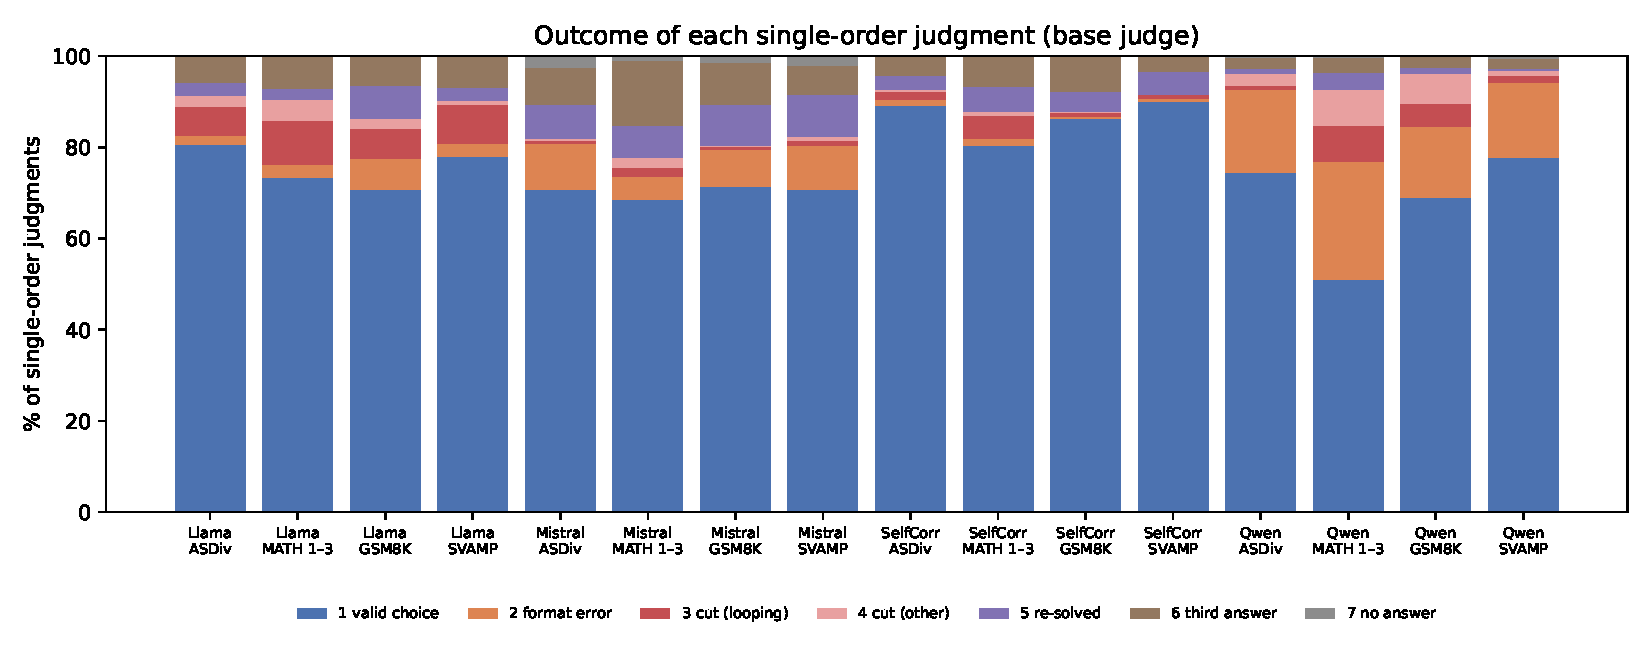
\includegraphics[width=\linewidth]{figures/invalid_types_base.pdf}
\caption{Outcome of each single-order judgment (\texttt{base} judge, one-right pairs, both orders), 16 grid
cells. Exploratory classification; rules fixed before the analysis.}
\label{fig:types}
\end{figure}

\paragraph{Decomposing the gap.} Let $R=\sigma(\delta)$ be the accuracy of a judge with the estimated skill
$\delta$, no position bias and no invalid choices ($\delta$ and bias $\beta$ fitted on valid judgments only).
We split the gap between $R$ and single-order accuracy into four factors with Shapley values over the 24
removal orders: position bias, format errors (class 2), truncation (3--4), and no choice despite a finished
output (5--7). Table~\ref{tab:decomp} gives the split. In the 16 grid cells the gap is 6.4--43.3 points; position
bias accounts for 0.0--2.5 of it, and the three invalid-choice factors for the rest: format errors 0.2--22.8
(largest for Qwen), truncation 0.5--13.9 (largest for Llama and for Qwen on MATH), and no choice 2.6--16.4
(largest for Mistral). With \texttt{base\_c} the gap shrinks to 2.1--13.6 points.

\begin{table}[t]
\centering\small
\caption{Four-factor Shapley split of the gap $R-$single-order accuracy (\texttt{base} judge, points).
``Valid'' = share of judgments with a valid choice. Gap with 95\% problem-clustered bootstrap CI. Exploratory.}
\label{tab:decomp}
\begin{tabular}{llrrrrrrr}
\toprule
Model & Dataset & Valid & Single & Gap [CI] & Bias & Format & Cut & No choice \\
\midrule
Llama-3.1-8B & ASDiv & 80.7 & 57.3 & 14.3 [11.5, 17.5] & 0.4 & 1.3 & 6.2 & 6.3 \\
 & MATH 1--3 & 73.3 & 53.0 & 19.4 [16.9, 22.3] & 0.2 & 2.1 & 10.3 & 6.9 \\
 & GSM8K & 70.8 & 50.2 & 21.3 [17.8, 25.5] & 0.6 & 4.7 & 6.3 & 9.7 \\
 & SVAMP & 77.9 & 56.4 & 16.7 [13.9, 19.6] & 0.6 & 2.1 & 6.8 & 7.1 \\
Mistral-7B & ASDiv & 70.8 & 51.3 & 21.3 [18.8, 23.9] & 0.1 & 7.3 & 0.8 & 13.0 \\
 & MATH 1--3 & 68.6 & 50.5 & 23.5 [20.1, 27.0] & 0.5 & 3.6 & 3.1 & 16.4 \\
 & GSM8K & 71.3 & 47.4 & 19.4 [16.7, 22.2] & 0.3 & 5.4 & 0.5 & 13.1 \\
 & SVAMP & 70.8 & 47.4 & 19.6 [17.6, 22.0] & 0.1 & 6.4 & 1.3 & 11.8 \\
Self\_Correction & ASDiv & 89.1 & 55.9 & 6.9 [5.2, 8.6] & 0.0 & 0.8 & 1.4 & 4.6 \\
 & MATH 1--3 & 80.4 & 49.0 & 11.9 [10.0, 14.1] & 0.1 & 0.9 & 3.5 & 7.4 \\
 & GSM8K & 86.3 & 52.2 & 8.5 [6.9, 10.5] & 0.2 & 0.2 & 0.7 & 7.4 \\
 & SVAMP & 90.0 & 56.3 & 6.4 [5.0, 7.9] & 0.2 & 0.4 & 0.5 & 5.4 \\
Qwen2.5-7B-Instr. & ASDiv & 74.4 & 63.5 & 23.7 [20.2, 28.5] & 2.3 & 15.2 & 3.0 & 3.3 \\
 & MATH 1--3 & 50.9 & 45.1 & 43.3 [39.1, 48.2] & 0.2 & 22.8 & 13.9 & 6.5 \\
 & GSM8K & 68.9 & 56.4 & 25.8 [22.0, 30.0] & 0.5 & 12.5 & 9.7 & 3.0 \\
 & SVAMP & 77.8 & 63.1 & 20.0 [17.1, 23.0] & 2.5 & 12.8 & 2.1 & 2.6 \\
\bottomrule
\end{tabular}

\end{table}

\paragraph{Sensitivity.} The split does not hinge on the logistic model. (i) In a model-free view,
single-order accuracy equals $(1-\pi)\,\mathrm{acc}_{AB}$, with $\pi$ the invalid share and
$\mathrm{acc}_{AB}$ the accuracy of valid judgments; this identity holds to machine precision in every cell.
The Shapley share of invalid choices always lies above the lower bound $0.5\pi$ (invalid judgments would have
been coin flips). It equals the upper bound $\pi\,\mathrm{acc}_{AB}$ to within 0.1 points (invalid judgments
would have been as accurate as valid ones). (ii) Replacing the logistic link with a probit changes the bias
share by at most 0.6 points; the largest bias share under probit is 1.9 points, inside the preregistered
3-point criterion. (iii) The separation is not fully clean for Qwen. Its invalid share depends on where the
correct solution sits: it is 7--18 points higher when the correct solution is second, with CIs excluding 0 in
5/5 Qwen cells and in Llama MATH. So for Qwen part of the position preference shows up as failing to choose,
not as a wrong choice.

The token cap is not the cause: re-judging Llama's endpoint pairs with a 1536-token cap lowers the share of
truncated judgments (18.1\% $\to$ 12.8\% on ASDiv, 31.9\% $\to$ 15.8\% on MATH) but leaves the gap unchanged (14.3 $\to$ 14.5 points on ASDiv, 19.4 $\to$ 19.6 on MATH);
the extra tokens end in an output that still names neither solution, consistent with most truncated judgments
being loops.

\subsection{Order averaging adds little (comparison with Ren et al.)}
Table~\ref{tab:ren} compares order averaging on the scale of \citet{ren2023selfeval}. \textbf{E2 passes in
1/4 endpoint cells} (Llama MATH $+5.0$ [0.9, 9.3]; others $+0.6$, $+0.7$, $+3.3$ with CIs including 0). The
bias-removal part of the gain is near 0 in every endpoint cell although the log-odds bias toward position A is
large (1.3--2.4); the preregistered prediction that this part grows with $|$bias$|$ is not supported
($\rho=-0.20$ over 4 cells, $-0.27$ over 16). In descriptive cells the gain is heterogeneous (0--11 points;
8/16 cells $\geq$3 points with CI above 0), and mostly comes from reading two orders rather than removing a
bias. Note that tie-break minus single-order accuracy is \emph{not} a debiasing gain: per pair it equals half
the indicator that no order picks the right solution and at least one invents an answer
(Appendix~\ref{app:identity}).

\begin{table}[t]
\centering\small
\caption{Single-order vs order-averaged verdict accuracy (\texttt{base\_c} log-probabilities), same scale as
\citet{ren2023selfeval}. Gain with 95\% CI.}
\label{tab:ren}
\resizebox{\linewidth}{!}{\begin{tabular}{lllrl}
\toprule
Study / model & Dataset & Single $\to$ averaged & Gain [CI] & Bias removal \\
\midrule
Ren et al., PaLM-2 L & TruthfulQA & 58.3 $\to$ 58.9 & +0.6 & --- \\
Ren et al., PaLM-2 L & TL;DR & 70.2 $\to$ 70.7 & +0.5 & --- \\
\textbf{Llama-3.1-8B} & ASDiv & 61.8 $\to$ 62.4 & +0.6 [$-$3.7, 4.8] & $-$0.8 \\
 & MATH 1--3 & 62.4 $\to$ 67.4 & \textbf{+5.0} [0.9, 9.3] & +1.4 \\
\textbf{Mistral-7B} & ASDiv & 71.7 $\to$ 72.4 & +0.7 [$-$2.3, 3.6] & $-$0.3 \\
 & MATH 1--3 & 62.7 $\to$ 66.0 & +3.3 [$-$0.7, 7.3] & +1.2 \\
Self\_Correction & GSM8K (report pairs) & 56.7 $\to$ 64.9 & +8.2 [3.6, 12.8] & +2.2 \\
Qwen2.5-7B-Instr. & ASDiv / MATH / GSM8K / SVAMP & 55--59 $\to$ 57--63 & $-$0.2 to +6.0 & $-$0.8 to +2.7 \\
\bottomrule
\end{tabular}}
\end{table}

\subsection{Hidden states}
A linear probe (standardized features, L2 logistic regression, $C=0.01$, layer chosen by grouped CV on the
training set) reads which solution is right from the last token of the judge prompt in all four models
(cross-dataset AUC 0.66--0.90). The probe beats a surface-feature baseline (length, step count, answer
magnitude) in every train/test direction only for Self\_Correction (e.g.\ 0.814 vs 0.690 for SVAMP$\to$GSM8K);
for Llama only on the endpoint datasets; for Mistral and Qwen surface features are stronger (Qwen 0.91--0.95,
likely the answer-format artefact). A pointwise probe that scores one solution at a time is stronger than the
pairwise probe (AUC 0.69--0.97). No probe is order-invariant: its choice flips with the order in 22--72\% of
pairs. Log-probability of the solution is a weak selector (48--69\%).

\paragraph{Probe-weighted voting out of sample (exploratory).} We trained a pointwise probe on the
answer-site state of $s_1$--$s_3$ on one dataset and used it on another. Each answer cluster was weighted by the
summed probe probability, and the heaviest cluster was chosen. Three train$\to$test pairs were used
(ASDiv$\to$MATH, MATH$\to$ASDiv, SVAMP$\to$GSM8K). The criterion, fixed before running, was a paired CI above
0 in at least 2/3 pairs. Weighted voting beats vote@3 by $+1.7$ to $+3.4$ points for Llama (2/3 pairs) and by
$+3.2$ to $+4.4$ for Mistral (3/3), so it is confirmed out of sample for these two models. It is not confirmed
for Self\_Correction (1/3; $+0.6$ to $+3.4$) or for Qwen (0/3; $-1.1$ to $+1.6$), whose vote@3 is already
high. The test AUC is 0.77--0.90 in all models. The gains are smaller than the gap between vote@3 and
vote@5, and we cannot test a probe-weighted vote@5 because no hidden states were saved for $s_4$--$s_5$.

\subsection{Practical value}
Table~\ref{tab:practical} and Figure~\ref{fig:practical} compare strategies by accuracy per problem and
mean number of model calls. The judge is called only when $s_1\neq s_2$ (22--87\% of problems), in both orders,
so it costs $2+2P(s_1\neq s_2)$ = 2.4--3.7 calls. Taking the judge's consistent choice, and otherwise a random
one, \emph{loses} to three-sample voting by 1.7--9.6 points, with the paired CI below 0 in 15/16 cells (13/16
under the rescued reading). Self-check, which falls back to a third sample when the two orders disagree, is
within $-2.4$ to $+1.1$ points of vote@3 (CI above 0 in no cell) at 2.6--4.4 calls. Agreement-gated voting
(stop if $s_1=s_2$) gives exactly the vote@3 answer at 2.2--2.9 calls, and is the cheapest way to get it.
Five-sample voting beats every two-candidate strategy in 15--16/16 cells. Even a perfect arbiter could not
change this much: 20--76\% of disagreements have both solutions wrong, so the ceiling (correct if $s_1$ or
$s_2$ is correct) is at most 1.6 points above vote@5, and not above it in 8/16 cells.

\begin{table}[t]
\centering\small
\caption{Accuracy (\%) per problem, project parser. Judge = consistent choice over both orders, otherwise
random; self-check = otherwise vote@3. Ceiling = $s_1$ or $s_2$ correct. Paired bootstrap CI. Exploratory.}
\label{tab:practical}
\resizebox{\linewidth}{!}{\begin{tabular}{llrrrrrrr}
\toprule
Model & Dataset & Keep $s_1$ & Judge & Self-check & vote@3 & vote@5 & Ceiling & Judge $-$ vote@3 [CI] \\
\midrule
Llama-3.1-8B & ASDiv & 79.6 & 81.8 & 83.8 & 83.7 & 87.1 & 88.0 & $-$1.9 [$-$3.5, $-$0.4] \\
 & MATH 1--3 & 44.2 & 47.4 & 51.5 & 50.8 & 57.3 & 57.8 & $-$3.4 [$-$5.5, $-$1.4] \\
 & GSM8K & 74.3 & 74.2 & 78.3 & 78.3 & 82.4 & 83.6 & $-$4.0 [$-$6.1, $-$1.9] \\
 & SVAMP & 75.7 & 78.6 & 81.1 & 80.8 & 84.9 & 86.5 & $-$2.2 [$-$3.8, $-$0.6] \\
Mistral-7B & ASDiv & 54.6 & 61.6 & 68.1 & 68.5 & 75.3 & 74.9 & $-$6.9 [$-$9.1, $-$4.7] \\
 & MATH 1--3 & 15.8 & 22.1 & 25.0 & 23.8 & 28.8 & 30.1 & $-$1.7 [$-$3.8, 0.3] \\
 & GSM8K & 43.1 & 48.3 & 54.9 & 55.6 & 65.1 & 64.5 & $-$7.3 [$-$10.3, $-$4.4] \\
 & SVAMP & 51.8 & 58.6 & 65.4 & 66.2 & 75.0 & 74.0 & $-$7.6 [$-$9.9, $-$5.5] \\
Self\_Correction & ASDiv & 79.6 & 81.1 & 83.5 & 85.6 & 88.3 & 88.8 & $-$4.5 [$-$6.2, $-$2.8] \\
 & MATH 1--3 & 50.2 & 50.8 & 54.0 & 56.4 & 61.4 & 62.4 & $-$5.7 [$-$8.0, $-$3.4] \\
 & GSM8K & 65.8 & 66.5 & 69.5 & 71.1 & 76.8 & 76.8 & $-$4.6 [$-$7.0, $-$2.2] \\
 & SVAMP & 82.7 & 83.5 & 85.4 & 87.0 & 90.3 & 91.6 & $-$3.4 [$-$5.1, $-$1.8] \\
Qwen2.5-7B-Instr. & ASDiv & 85.6 & 87.5 & 91.6 & 91.0 & 92.7 & 92.5 & $-$3.5 [$-$4.7, $-$2.2] \\
 & MATH 1--3 & 55.9 & 57.0 & 66.4 & 66.6 & 71.3 & 66.8 & $-$9.6 [$-$11.4, $-$7.9] \\
 & GSM8K & 81.1 & 81.3 & 85.4 & 84.7 & 89.1 & 88.6 & $-$3.4 [$-$5.2, $-$1.5] \\
 & SVAMP & 85.0 & 86.3 & 90.4 & 90.1 & 92.7 & 92.6 & $-$3.8 [$-$5.2, $-$2.4] \\
\bottomrule
\end{tabular}
}
\end{table}

\begin{figure}[t]
\centering
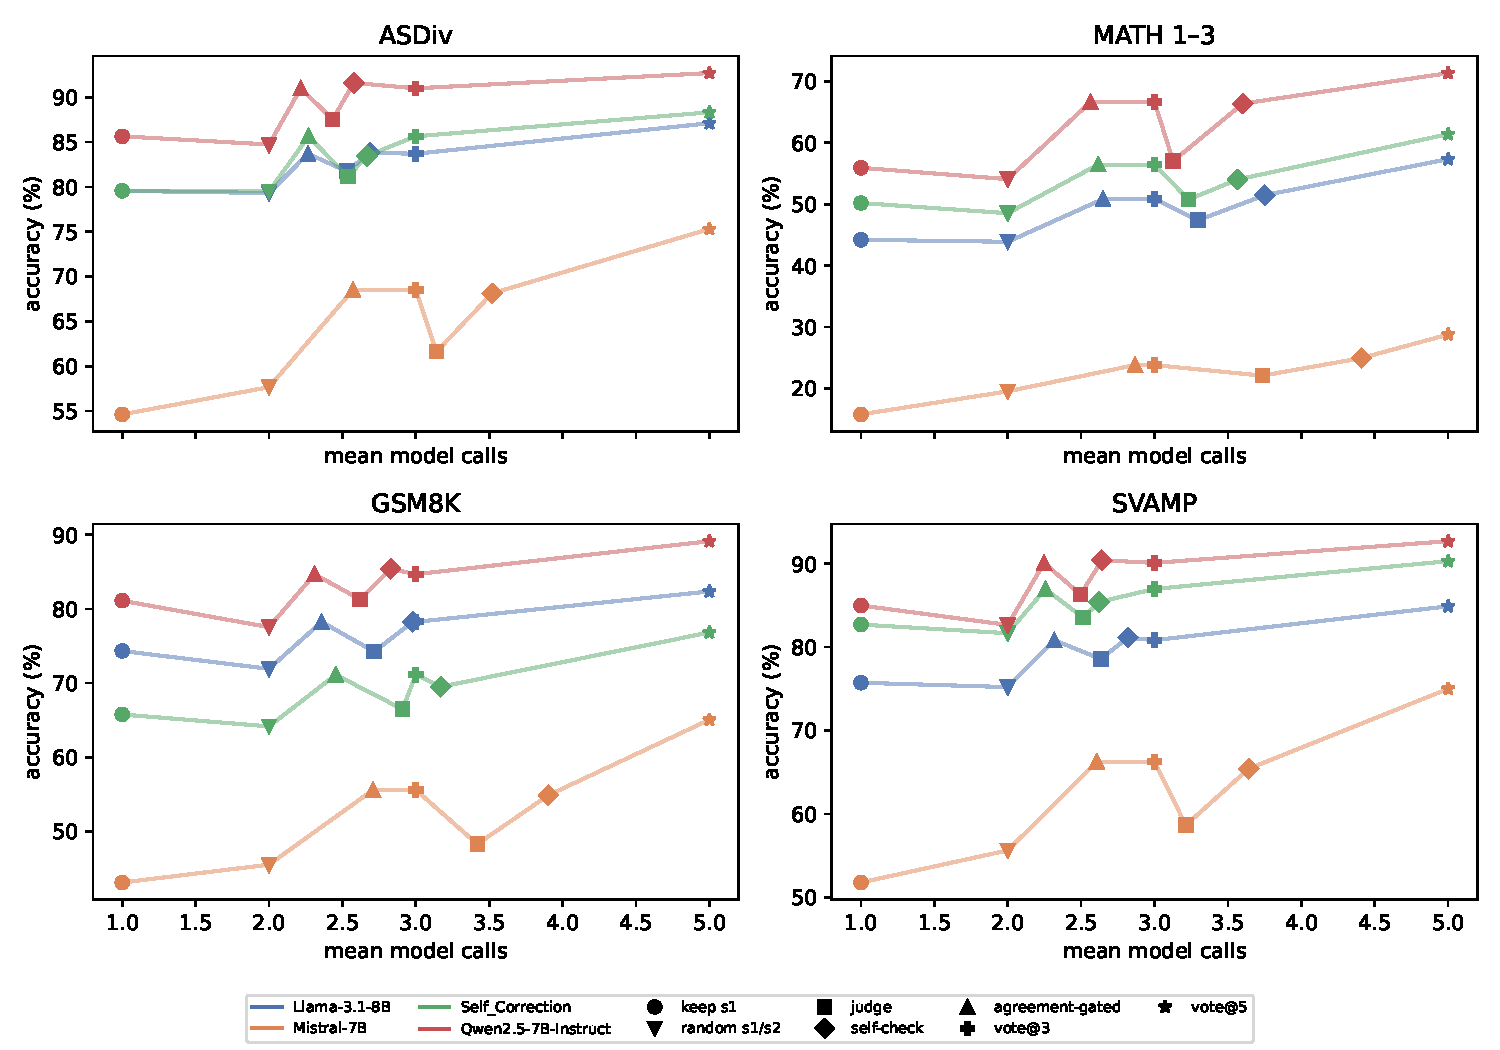
\includegraphics[width=\linewidth]{figures/practical_calls.pdf}
\caption{Accuracy vs mean model calls per problem, one panel per dataset; colors are models, markers are
strategies.}
\label{fig:practical}
\end{figure}

\subsection{A closer look at the self-correction model}\label{sec:sc}
On the original GSM8K pairs the untrained judge has skill index $+0.215$ [0.128, 0.304] and tie-break 0.601;
order-swapped DPO raises tie-break by 5.2 points (Holm $p=0.016$) and cuts invented answers from 16.7\% to
2.1\%, while a probe trained on the same states is unchanged across all four judges (65--69\%): training
changes how the signal is expressed, not the signal. The Phase-14 pipeline reproduces every number of this
analysis exactly from the saved outputs, and a fresh sample reproduces it within its CI (skill 0.191).

\section{Discussion}
\paragraph{What makes arbitration look like guessing.} Position bias is real and model-specific, but costs
little accuracy because a moderate symmetric bias reduces accuracy only to second order. The large cost is the
judge failing to commit to one of the two solutions. For instruction models this is partly a reading problem
(answers written as sentences); for the others it is invented third answers or loops cut by the token limit.
\paragraph{A weak point: Qwen.} The decomposition assumes that how often a judge fails to choose does not
depend on where the correct solution is shown. This holds in 15 of 21 cells but not for Qwen: its invalid
share is 7--18 points higher when the correct solution is second (CIs excluding 0 in all 5 Qwen cells, and
in Llama MATH). For these cells part of the position preference is expressed as a failure to choose rather
than a wrong choice, so the bias share in Table~\ref{tab:decomp} is a lower bound and the invalid-choice
share an upper bound. The conclusion that bias costs little is weakest for Qwen.
\paragraph{Parent vs fine-tuned model (open question).} The untrained parent has a 2--3$\times$ larger skill
index than the self-correction model on all four datasets, and the gap widens under the rescued reading. Each
model judges its own pairs, which differ in difficulty, so we do not claim that self-correction SFT reduces
arbitration skill; testing this needs both models to judge the same pairs.
\paragraph{Recommendation.} When a model arbitrates its own solutions, swap-test, report single-order accuracy
together with the skill index and tie-break, and report how often the judge fails to make a valid choice.

\section{Limitations}
Endpoints cover two models $\times$ two datasets; the other cells are descriptive and were generated after the
endpoints were opened. All prompts are in Vietnamese; Mistral is a weak solver here and often answers in
English. The project parser misreads answers written as sentences. Judges decode greedily without a
repetition penalty, which affects looping. Log-probabilities exist only for the constrained judge and cover
50--94\% of pairs. For Qwen the invalid share depends on the position of the correct solution, so the
separation of position bias from invalid choices is not fully clean for that model. The check of the rescued
reading was done by the analysing assistant, not by an independent annotator. One run per cell. Llama weights come from a byte-identical public copy of Meta's
release. Most analyses beyond E1/E2 are post hoc and need confirmation on new data.

\section{Conclusion}
Measured in one order, a 7B model arbitrating between its own conflicting solutions looks like it is guessing.
Decomposed, the skill is real and general across model families and datasets; the shortfall comes mostly from
the judge not making a valid choice, and only a little from position bias. Constraining the output format removes most
invalid choices. Order averaging adds little, and at the system level self-arbitration does not beat majority
voting.

\paragraph{Data and code availability.} All numbers in this paper are recomputed on CPU from saved model
outputs; generation used one rented GPU. Analysis scripts, saved outputs, the data catalog with SHA-256 hashes,
and the preregistration with every amendment are in the project repository,
\url{https://github.com/KhangTranManh/Self-Correction-Model}
(archived version: \href{https://doi.org/10.5281/zenodo.23541462}{doi:10.5281/zenodo.23541462}).

\bibliographystyle{plainnat}
\bibliography{refs}

\appendix
\section{Data integrity and counts}
Table~\ref{tab:counts} lists the counts for every cell after filtering. Of the 561 GSM8K problems, 42 had
appeared in an earlier evaluation run (not in any training data). Excluding them leaves 519 problems and does
not change any conclusion: skill index 0.320 (Llama), 0.249 (Mistral), 0.186 (Self\_Correction), 0.487 (Qwen)
(\texttt{report.json}, key \texttt{lenient\_audited}). ASDiv and MATH problems do
not overlap with data used in earlier phases. Bridge and report cells reuse the Phase-13/12 solutions of
Self\_Correction, which carry no token-cap flag (``---''); the two report cells also lack the cap flag for the
\texttt{base} judge.

\begin{table}[h]
\centering\scriptsize
\caption{Counts per cell. Cap columns: share (\%) of solutions hitting the 768-token cap and of judgments
hitting the judge cap (\texttt{base}, \texttt{base\_c}).}
\label{tab:counts}
\resizebox{\linewidth}{!}{\begin{tabular}{llrrrrrrrr}
\toprule
Model & Dataset & Problems & $s_1\neq s_2$ & Judged & One-right & Both wrong & Sol.\ cap & Judge cap & Judge\textsubscript{c} cap \\
\midrule
Llama-3.1-8B & ASDiv & 822 & 218 & 430 & 274 & 156 & 1.6 & 18.1 & 14.2 \\
 & MATH 1--3 & 785 & 509 & 1021 & 434 & 587 & 15.7 & 31.9 & 36.5 \\
 & GSM8K & 561 & 201 & 402 & 264 & 138 & 1.5 & 14.7 & 13.8 \\
 & SVAMP & 960 & 304 & 586 & 389 & 197 & 2.4 & 17.9 & 12.8 \\
 & Bridge & 561 & 240 & 486 & 288 & 198 & --- & 11.2 & 14.4 \\
Mistral-7B & ASDiv & 822 & 469 & 933 & 558 & 375 & 1.8 & 3.5 & 0.3 \\
 & MATH 1--3 & 785 & 681 & 1377 & 331 & 1046 & 15.8 & 16.9 & 1.6 \\
 & GSM8K & 561 & 398 & 780 & 411 & 369 & 2.1 & 3.7 & 0.1 \\
 & SVAMP & 960 & 582 & 1159 & 681 & 478 & 1.4 & 3.0 & 0.1 \\
 & Bridge & 561 & 240 & 486 & 288 & 198 & --- & 11.9 & 1.3 \\
Self\_Correction & ASDiv & 822 & 221 & 446 & 311 & 135 & 1.5 & 7.4 & 5.9 \\
 & MATH 1--3 & 785 & 483 & 970 & 452 & 518 & 9.0 & 15.0 & 14.4 \\
 & GSM8K & 561 & 255 & 493 & 277 & 216 & 1.7 & 3.9 & 3.3 \\
 & SVAMP & 960 & 246 & 500 & 371 & 129 & 1.2 & 3.2 & 2.5 \\
 & GSM8K (report) & 561 & 240 & 486 & 288 & 198 & --- & --- & 3.7 \\
 & SVAMP (report) & 960 & 246 & 501 & 367 & 134 & --- & --- & 3.2 \\
Qwen2.5-7B-Instr. & ASDiv & 822 & 178 & 361 & 256 & 105 & 0.6 & 9.6 & 1.8 \\
 & MATH 1--3 & 785 & 442 & 865 & 380 & 485 & 10.1 & 27.1 & 7.2 \\
 & GSM8K & 561 & 174 & 338 & 241 & 97 & 0.1 & 23.1 & 5.8 \\
 & SVAMP & 960 & 238 & 455 & 358 & 97 & 0.2 & 5.4 & 0.9 \\
 & Bridge & 561 & 240 & 486 & 288 & 198 & --- & 20.1 & 4.9 \\
\bottomrule
\end{tabular}
}
\end{table}

The \emph{rescued} reading was checked on a seeded sample of 179 class-2 judgments (50 per model; 29 available
for Self\_Correction). This check was done by the assistant that ran the analysis, not by an independent
annotator. Clear misreadings were 4/179 (2.2\%), all on answers that are not a single number (a root, a
fraction, two values). Counting ambiguous cases as errors gives 10.1\% overall: 0/50 for Qwen, 10\% for
Llama, 12\% for Mistral, and 24\% for Self\_Correction. Following the preregistered thresholds, the rescued
reading is the main sensitivity analysis for Qwen, is reported with a caveat for Llama and Mistral, and is
appendix-only for Self\_Correction.
\section{Self\_Correction deep dive}\label{app:sc}
All numbers are on the original GSM8K holdout (288 one-right pairs, both orders) unless noted.
\paragraph{Position split.} When the right solution is shown first, the untrained judge picks it 49.3\% of the
time (B: 34.4\%, invalid 16.3\%); when it is shown second, 55.2\% (A: 27.8\%, invalid 17.0\%). Skill index
$+0.215$ [0.128, 0.304], single-order accuracy 52.3\%. On SVAMP: skill $+0.248$ [0.166, 0.332].
\paragraph{Training the judge.} Order-swapped DPO (p12) raises tie-break from 0.601 to 0.653 (+5.2 points
[1.6, 8.8], Holm $p=0.016$); DPO on the constrained judge (p13b) beats the constrained baseline by 8.3 points
(Holm $p=0.0008$) and cuts invalid choices from 4.9\% to 2.1\%. Consistent-only accuracy (71--79\%) overstates
quality: over all one-right pairs the best judge is right on 41--47\% and inconsistent on about half.
\paragraph{Is the judge better than random?} Choosing between $s_1$ and $s_2$ at random is no better than
keeping $s_1$ (65.7 vs 66.1\% on GSM8K). The trained judge adds 4.2 points over random choice on GSM8K and 3.1
on SVAMP; a self-check that falls back to a third sample reaches vote@3 (72.2 vs 72.0\%) but not vote@5 (77.5\%).
\paragraph{Hidden states.} With one protocol for all four judges, a linear probe on the judge-prompt state
reaches 65--69\% across datasets (SVAMP$\to$GSM8K) and $\approx$71.5\% within GSM8K, with no effect of judge
training. Surface features alone reach AUC 0.742; hidden + surface 0.759, and the probe is right on 64\% of
the rows where surface features fail, so the two signals are only partly distinct. The probe is not
order-invariant (about 44\% of pairs flip). Mean token log-probability selects the right solution 56--61\% of
the time; agreement with one extra greedy solve reaches 81\% but costs a solver call. A logit lens on the
verdict letter becomes informative only from layer $\approx$22, several layers after the linear probe.
\paragraph{Origin of the second-position preference.} Every row of the self-correction SFT format is a
failed attempt followed by the verified correction, so the data carry a ``later answer is right'' prior by
construction; this is \emph{consistent with} the preference but does not show that it caused it. Renaming
the labels (first shown called ``Solution B'') leaves the preference unchanged, so it follows position, not
the label. Restating the problem after the solutions removes the net preference ($+0.090\to+0.009$) and raises
coverage, but not accuracy (nominal $p=0.04$, not significant after Holm).

\section{Bridge set and parent-model checks}
Four judges re-judged the same 288 GSM8K pairs written by Self\_Correction (bridge set). Tie-break: Qwen-Instruct
0.774, Llama 0.729, Mistral 0.595, Self\_Correction itself 0.601. Qwen-Instruct shows no net position
preference here ($-0.024$ [$-0.073$, 0.026]). This gap is \emph{not} evidence that SFT harmed arbitration.
On its own conflicting solutions the parent reaches only 0.61--0.66, it prefers the first position, and the
two sets of pairs differ in difficulty. A stronger judge does well on a weaker model's disagreements.

\section{Truncation labels and token-cap sensitivity}
Every output that hit its token cap was labelled automatically, in a fixed order: (c) off-topic, garbage or a
language switch; (b) looping (a 10-word sequence or a sentence repeated verbatim $\geq$3 times, or a templated
list); (d) for judgments only, abandoning both solutions and re-solving; (a) otherwise, still on track. Loops
dominate the capped judgments of Llama (65--91\% of its capped \texttt{base} judgments in the four grid
datasets) and Self\_Correction (73--100\% in the pilot). Mistral and Qwen also re-solve or are cut while still on track. Raising Llama's cap
to 1536 tokens lowers the capped share (18.1\% $\to$ 12.8\% on ASDiv, 31.9\% $\to$ 15.8\% on MATH), but 74--76\%
of the outputs still capped are loops, and the single-order gap does not shrink (Section~\ref{sec:decomp}). Full tables:
\texttt{paper/results/phase14\_truncation.md}.
\section{Tie-break identity}\label{app:identity}Per pair, tie-break minus mean
single-order accuracy equals
\[\tfrac12\,\mathbf{1}\bigl[\text{no order picks the right solution and one order gives a third answer}\bigr];\]
a judge with pure position bias and no invalid choices gets 0.
\section{Prompts, hyperparameters, code and hashes}See \nolinkurl{phase14/DATA_CATALOG.md} and \nolinkurl{phase14/DATA_MANIFEST.json} in the repository.

\end{document}
